\documentclass{report}
\usepackage[utf8]{inputenc}
\usepackage{blindtext}
\usepackage[T1]{fontenc}
\usepackage{graphicx}
\usepackage[margin=0.75in]{geometry}
\usepackage{hyperref}
\usepackage{amsmath}
\usepackage{enumitem}
\usepackage{wrapfig}
\usepackage{multicol}
\graphicspath{ {../assets/} }

\newlist{choices}{enumerate}{1}
\setlist[choices]{label*=(\Alph*)}
\newcommand{\choice}{\item}

\SetEnumitemKey{twocol}{
  before=\raggedcolumns\begin{multicols}{2},
  after=\end{multicols}}

\SetEnumitemKey{threecol}{
  before=\raggedcolumns\begin{multicols}{3},
  after=\end{multicols}}

\title{
\centerline{
\includegraphics[width=50mm]{lymphad.jpg}}
\vspace{0.5cm}
Year 12 Physics - Mechanics\\
\vspace{0.5cm}
\large AS91171 \\ https://putaiao.nz/12phy/as91171/\\}
\author{Finn Le Sueur of Cashmere High School\\ \texttt{lsf@cashmere.school.nz}}
\date{2021}

\begin{document}

% Put title on own page
\maketitle

% Put contents on own page
\newpage
\tableofcontents

% ====================
%  Speed and Acceleration
% ====================
\newpage
\chapter{Speed and Acceleration}

\section{Warm Up}

\subsection{Pātai Tahi: Who is the fastest?}

\begin{enumerate}
\item Andy can run $100m$ in $11.9$ seconds
\item Bob can run $100m$ in $10.8$ seconds
\item Chris can run $100m$ in $12.4$ seconds
\end{enumerate}

\vspace{1cm}

\subsection{Pātai Rua: Who is the fastest?}

\begin{enumerate}
\item Aaron can run $534m$ in $1 minute$
\item Billy can run $510m$ in $1 minute$
\item Cameron can run $452m$ in $1 minute$
\end{enumerate}

\vspace{1cm}

\subsection{Pātai Toru: Who is the fastest?}

\begin{enumerate}
\item Ash can run $0.3km$ in $45 seconds$
\item Bailey can run $420m$ in $1 minute$
\item Caleb can run $510m$ in $1.5 minutes$
\end{enumerate}

\vspace{1cm}

\section{Formula: Average Speed}

\begin{align}
    v &= \frac{d}{t} \\
    d &= \text{total distance travelled} \\
    t &= \text{time} \\
    v &= \text{speed}
\end{align}

\subsection{What is the Unit?}

\begin{enumerate}
\item $ms^{-1}$
\item It stands for \textbf{meters per second}
\item E.g. the speed of sound is $343ms^{-1}$ - it travels at $343$ meters in one second
\end{enumerate}

\subsection{Example / Tauria}

Ash runs $315m$ in $45s$. Calculate his average speed in \textit{meters per second}.

\begin{enumerate}
\item Knowns
\item Unknowns
\item Formula 
\item Substitute
\item Solve
\end{enumerate}

\vspace {3cm}

\subsection{Pātai Tahi: Unit Conversions}

\begin{enumerate}
\item A skydiver (freefall) = $53ms^{-1}$
\item A handgun bullet = $660ms^{-1}$
\item A car on the road = $50km/hr$
\item A flying airplane = $1100kmh^{-1}$
\item Light = $300,000,000$
\end{enumerate}

In pairs, convert the speed of the car and airplane into \textit{meters per second}.

\vspace{3cm}

\subsection{Pātai Rua: Velocity Calculation}

A car is moving at a speed of $10ms^{-1}$. How far does the car travel in $12s$?

\begin{enumerate}
\item Knowns
\item Unknowns
\item Formula 
\item Substitute
\item Solve
\end{enumerate}

\vspace {3cm}

\subsection{Pātai Toru: Running Man}

A man is running at a speed of $4ms^{-1}$. How long does he take to run $100m$?

\begin{enumerate}
\item Knowns
\item Unknowns
\item Formula 
\item Substitute
\item Solve
\end{enumerate}

\vspace {3cm}

\section{Average vs Instantaneous Speed}

Velocity may refer to \textbf{average velocity} or \textbf{instantaneous velocity}. The formula $v = \frac{d}{t}$ can only be used to calculate \textbf{average velocity} or when \textbf{the velocity is constant} (acceleration is zero).

\section{Formula: Acceleration}

The rate of change in speed

\begin{align}
    a &= \frac{\Delta v}{t} \\
    \Delta v &= \text{ change in speed} \\
    t &= \text{ time} \\
    a &= \text{ acceleration}
\end{align}

\subsection{What Does $ms^{-2}$ Mean?}

\textbf{Whakatika}: meters per second squared OR meters per second per second. For example, $a=12ms^{-2}$ means that the velocity is increased by $12ms^{-1}$ every second.

\begin{table}[h]
\centering
\begin{tabular}{lllll}
\hline
Time ($s$)           & 0 & 1  & 2  & 3  \\ \hline
Velocity ($ms^{-1}$) & 0 & 12 & 24 & 36 \\ \hline
\end{tabular}
\end{table}

\subsection{Pātai: Re-arranging Acceleration}

Starting with $a = \frac{\Delta v}{t}$, re-arrange the equation for $v$ and $t$.

\begin{choices}[twocol]
   \choice $a = \frac{\Delta v}{t}$
   \choice $a = \frac{\Delta v}{t}$
\end{choices}

\vspace{3cm}

\section{Formula: Calculating Change ($\Delta$)}

This is the difference between the \textbf{initial} and the \textbf{final} value.

\begin{align}
    \Delta &= final - initial \\
    \text{e.g. }\Delta v &= v_{f} - v_{i}
\end{align}

\subsection{Pātai Whā: Walking}

A man initially walking at $2.0ms^{-1}$ notices that his house is on fire so he speeds up to $11ms^{-1}$ in $1.3s$.

\textbf{1. Calculate the change in speed}

\begin{enumerate}
\item Knowns
\item Unknowns
\item Formula 
\item Substitute
\item Solve
\end{enumerate}

\vspace {3cm}


\textbf{2. Calculate his acceleration}

\begin{enumerate}
\item Knowns
\item Unknowns
\item Formula 
\item Substitute
\item Solve
\end{enumerate}

\vspace {3cm}

\subsection{Pātai Rimu: The Car}

A car initially moving at $12.7ms^{-1}$ accelerates at $1.3ms^{-2}$ for \textbf{one minute}. What is the car's final speed?

\begin{enumerate}
\item Knowns
\item Unknowns
\item Formula 
\item Substitute
\item Solve
\end{enumerate}

\vspace{3cm}

\subsection{Pātai Ono: Decelerating Car}

A car decelerates at $1.8ms^{-2}$ for $9.4s$ to stop. What was the car's initial speed?

\begin{enumerate}
\item Knowns
\item Unknowns
\item Formula 
\item Substitute
\item Solve
\end{enumerate}

\vspace{3cm}

\newpage
\chapter{Vectors and Scalars}

\section{Introduction}

In pairs, think about and discuss the similarities and differences between these two questions:

\begin{enumerate}
    \item Mr Chu puts 40 apples inside a box, except Miss Nam eats two of them. What is the total number of apples inside the box?
    \item Mrs Carpenter lifts a plant off her desk with a force of $15N$ in the upwards direction, while the plant has a weight force of $5N$ acting down. What is the total force applied on the plant?
\end{enumerate}

\section{What is a Vector?}

\begin{itemize}
    \item \textbf{Scalar} = size only (e.g. mass)
    \item \textbf{Vector} = size + direction (e.g. velocity)
\end{itemize}

\subsection{Distance vs. Displacement}

\begin{itemize}
    \item \textbf{Distance} is the amount an object has moved
    \begin{itemize}
        \item It is a scalar
        \item e.g. $3km$
    \end{itemize}
    \item \textbf{Displacement} is the distance from start to finish in a straight line
    \begin{itemize}
        \item It is a vector, because direction is also important
        \item e.g. $3km$ South West
    \end{itemize}
\end{itemize}

\subsection{Pātai Tahi}

Ella drives to Sumner beach in the weekend because it is far too hot. She drives $5km$ south and $10km$ west to get there.

\textbf{1.} What is the total distance travelled by Ella?

\begin{itemize}
\item Knowns
\item Unknowns
\item Formula 
\item Substitute
\item Solve
\end{itemize}

\vspace{2cm}

\textbf{2.} What is the total displacement of Ella?

\begin{itemize}
\item Knowns
\item Unknowns
\item Formula 
\item Substitute
\item Solve
\end{itemize}

\vspace{2cm}

\subsection{Pātai Rua: Scalar or Vector}

Use the units to help you decide whether each is a scalar or a vector.

\begin{itemize}
    \item Distance
    \item Displacement
    \item Speed
    \item Velocity
    \item Acceleration
    \item Momentum
    \item Energy
    \item Force
    \item Temperature
    \item Mass
    \item Work
    \item Power
\end{itemize}

\subsection{Vectors}

When dealing with problems which involve vector quantities (e.g. calculating velocity, force, etc.), you must consider the size and direction.

Which means: \textbf{you must use vector calculations and/or vector diagrams.}

\begin{itemize}
    \item Have both \textbf{direction} and \textbf{magnitude}
    \item Drawn as an arrow
    \item Drawn with a ruler
    \item Drawn to scale (on a grid, typically)
    \item Drawn head-to-tail
    \item Can be added an subtracted
    \item Use Pythagoras and SOH CAH TOA to find values
\end{itemize}

\begin{wrapfigure}{r}{0.25\textwidth}
    \centering
    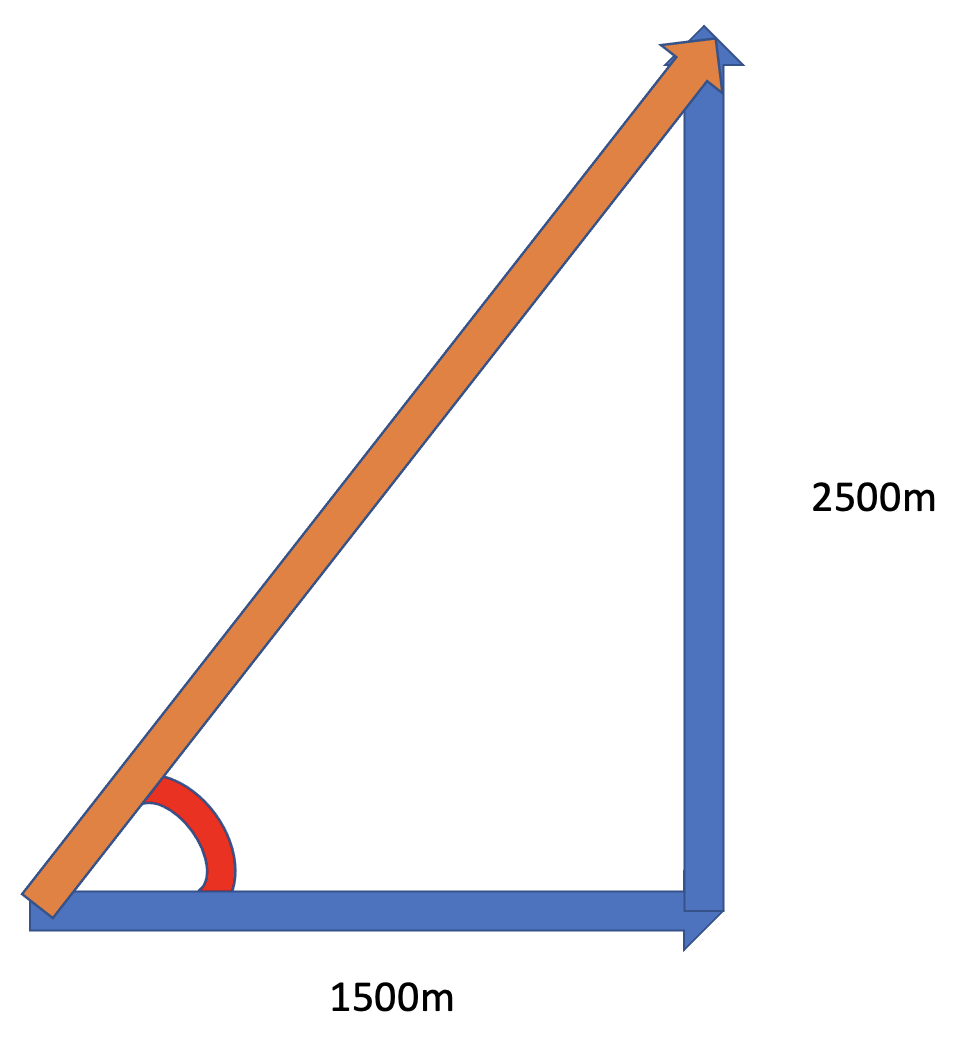
\includegraphics[width=0.25\textwidth]{trigonometry.png}
\end{wrapfigure}

\newpage
\chapter{Kinematic Equations}

\newpage
\chapter{Newton's Laws}

\newpage
\chapter{Projectile Motion}

\newpage
\chapter{Torque and Equilibrium}

\newpage
\chapter{Circular Motion}

\newpage
\chapter{Momentum and Impulse}

\newpage
\chapter{Energy, Work, and Power}

\end{document}